%%%%%%%%%%%%%%%%%%%%%%%%%%%%%%%%%%%%%%%%%%%%%%%%%%%%%%%%%%%
% --------------------------------------------------------
% Tau
% LaTeX Template
% Version 2.4.4 (28/02/2025)
%
% Author: 
% Guillermo Jimenez (memo.notess1@gmail.com)
% 
% License:
% Creative Commons CC BY 4.0
% --------------------------------------------------------
%%%%%%%%%%%%%%%%%%%%%%%%%%%%%%%%%%%%%%%%%%%%%%%%%%%%%%%%%%%

\documentclass[9pt,a4paper,column,twoside]{tau-class/tau}
\usepackage[english]{babel}

%% Spanish babel recomendation
% \usepackage[spanish,es-nodecimaldot,es-noindentfirst]{babel} 

%% Draft watermark
% \usepackage{draftwatermark}

%----------------------------------------------------------
% TITLE
%----------------------------------------------------------

\journalname{Intro Microelectronic Circuits with Laboratory}
\title{Resistors and Bipolar Transistors}

%----------------------------------------------------------
% AUTHORS, AFFILIATIONS AND PROFESSOR
%----------------------------------------------------------

\author[1]{Anika Mahesh}
\author[1]{Elias Tuthill}
\author[1]{Henry Tejada Deras}

%----------------------------------------------------------

\affil[1]{Franklin W. Olin College of Engineering}

%----------------------------------------------------------
% FOOTER INFORMATION
%----------------------------------------------------------

\institution{Franklin W. Olin College of Engineering}
\footinfo{Intro Microelectronic Circuits with Laboratory}
\theday{TBD}
\leadauthor{Mahesh et. al.}

%----------------------------------------------------------

\begin{document}
		
    \maketitle 
    \thispagestyle{firststyle} 
    % \tauabstract 
    % \tableofcontents
    % \linenumbers 
    
%----------------------------------------------------------

\section{Bipolar Transistor Characteristics}
	\subsection{Results}
	\begin{figure}[H]
 		\centering
   		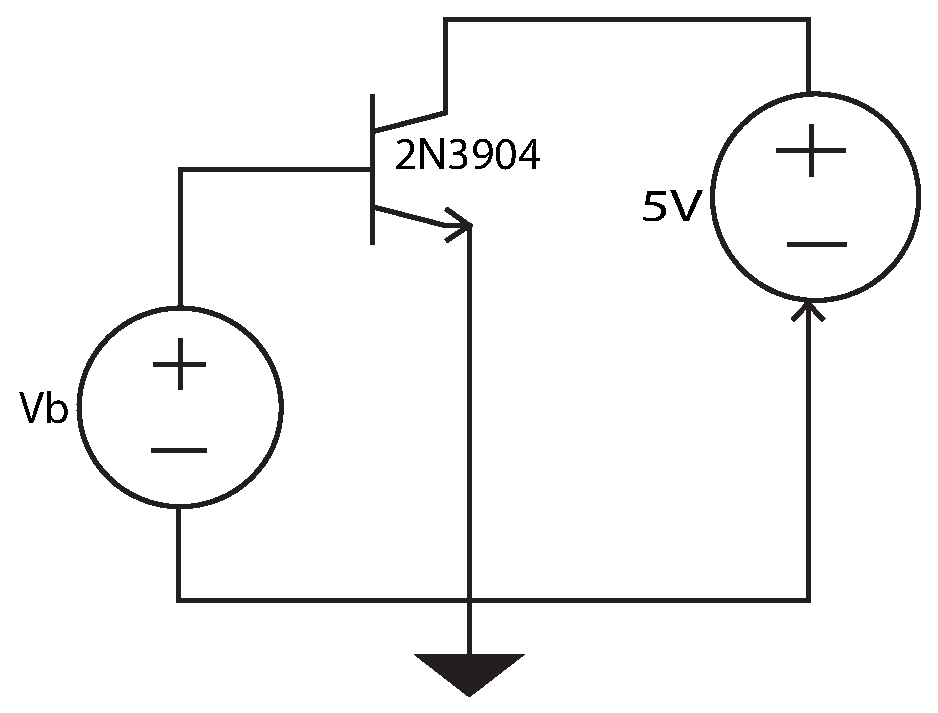
\includegraphics[width=0.6\linewidth]{../diagrams/lab3_c1.pdf}
   		\caption{The schematic for the experimental setups used in Experiment 1.}\label{fig:exp2_diag}
    \end{figure}
	\subsection{Analysis}
	\subsection{Discussion}
\section{Emitter-Degenerated Bipolar Characteristics}
	\subsection{Results}
	\begin{figure}[H]
 		\centering
   		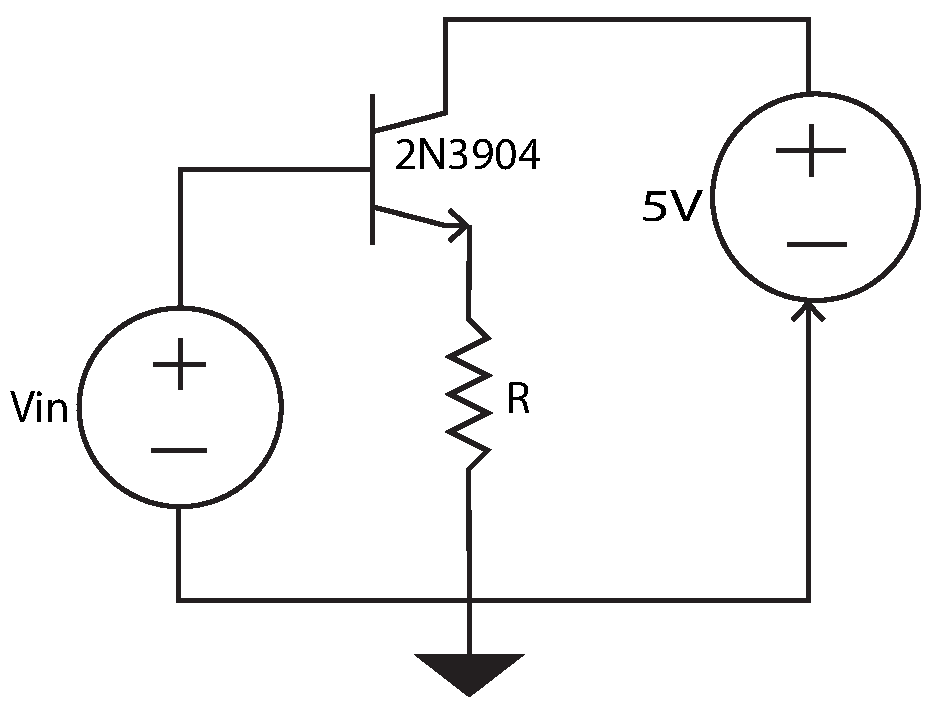
\includegraphics[width=0.6\linewidth]{../diagrams/lab3_c2.pdf}
   		\caption{The schematic for the experimental setups used in Experiment 2.}\label{fig:exp2_diag}
    \end{figure}
	\subsection{Analysis}
	\subsection{Discussion}
\section{Follower Voltage Transfer Characteristics}
	\subsection{Results}
	\begin{figure}[H]
 		\centering
   		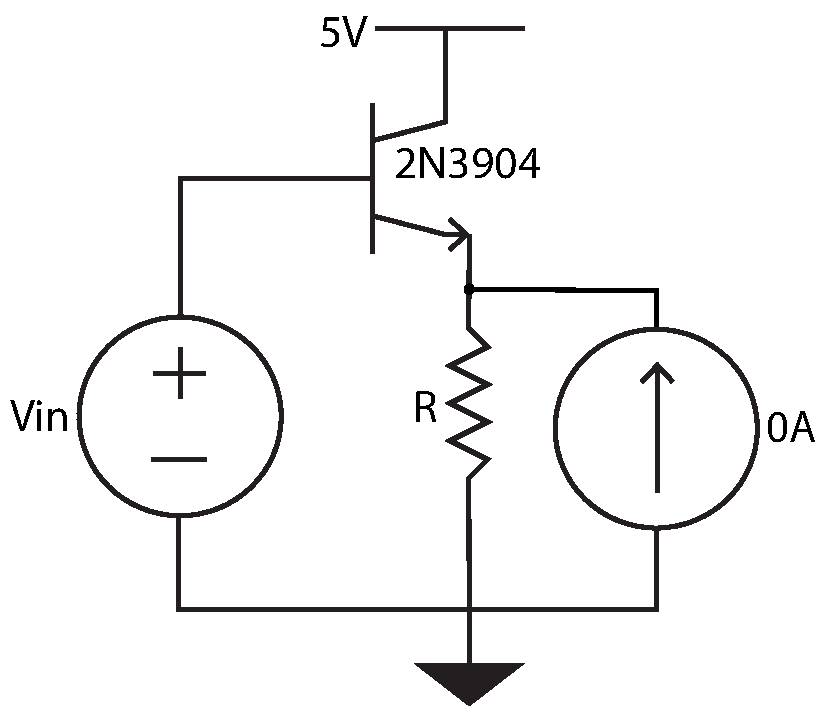
\includegraphics[width=0.6\linewidth]{../diagrams/lab3_c3.pdf}
   		\caption{The schematic for the experimental setups used in Experiment 3.}\label{fig:exp2_diag}
    \end{figure}
	\subsection{Analysis}
	\subsection{Discussion}
\section{Inverter Voltage Transfer Characteristics}
	\subsection{Results}
	\begin{figure}[H]
 		\centering
   		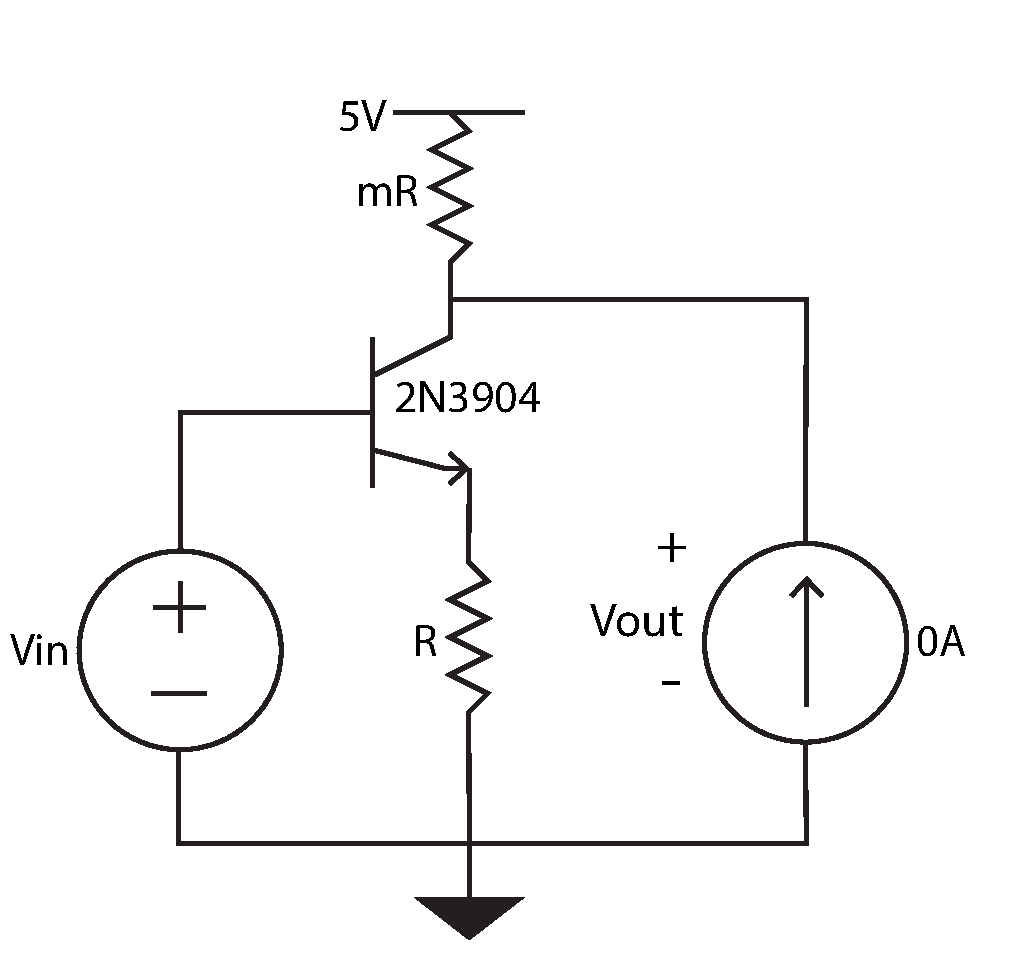
\includegraphics[width=0.6\linewidth]{../diagrams/lab3_c4.pdf}
   		\caption{The schematic for the experimental setups used in Experiment 4.}\label{fig:exp2_diag}
    \end{figure}
	\subsection{Analysis}
	\subsection{Discussion}

%----------------------------------------------------------

\end{document}